\chapter{Capteur}

Ce project est basé sur l'utilisation du capteur Q-1 de la société openQCM.
L’openQCM Q-1 est un instrument de microbalance à quartz (Quartz Crystal Microbalance) capable de mesurer simultanément les variations de fréquence et de dissipation. 
L’appareil est donc capable de mesurer à la fois les variations de masse et les propriétés viscoélastiques du matériau à la surface du cristal de quartz.
Le capteur est open-source, sous la liscence creatve comon \cite{manual-openqcmQ1}.

Cette licence permet de partager le contenu et de l’adapter à condition que l’auteur soit crédité, que l’usage ne soit pas commercial, 
et que toute œuvre dérivée soit diffusée sous la même licence \cite{cc-by-nc-sa-4.0}.

\begin{figure}[H]
    \centering
    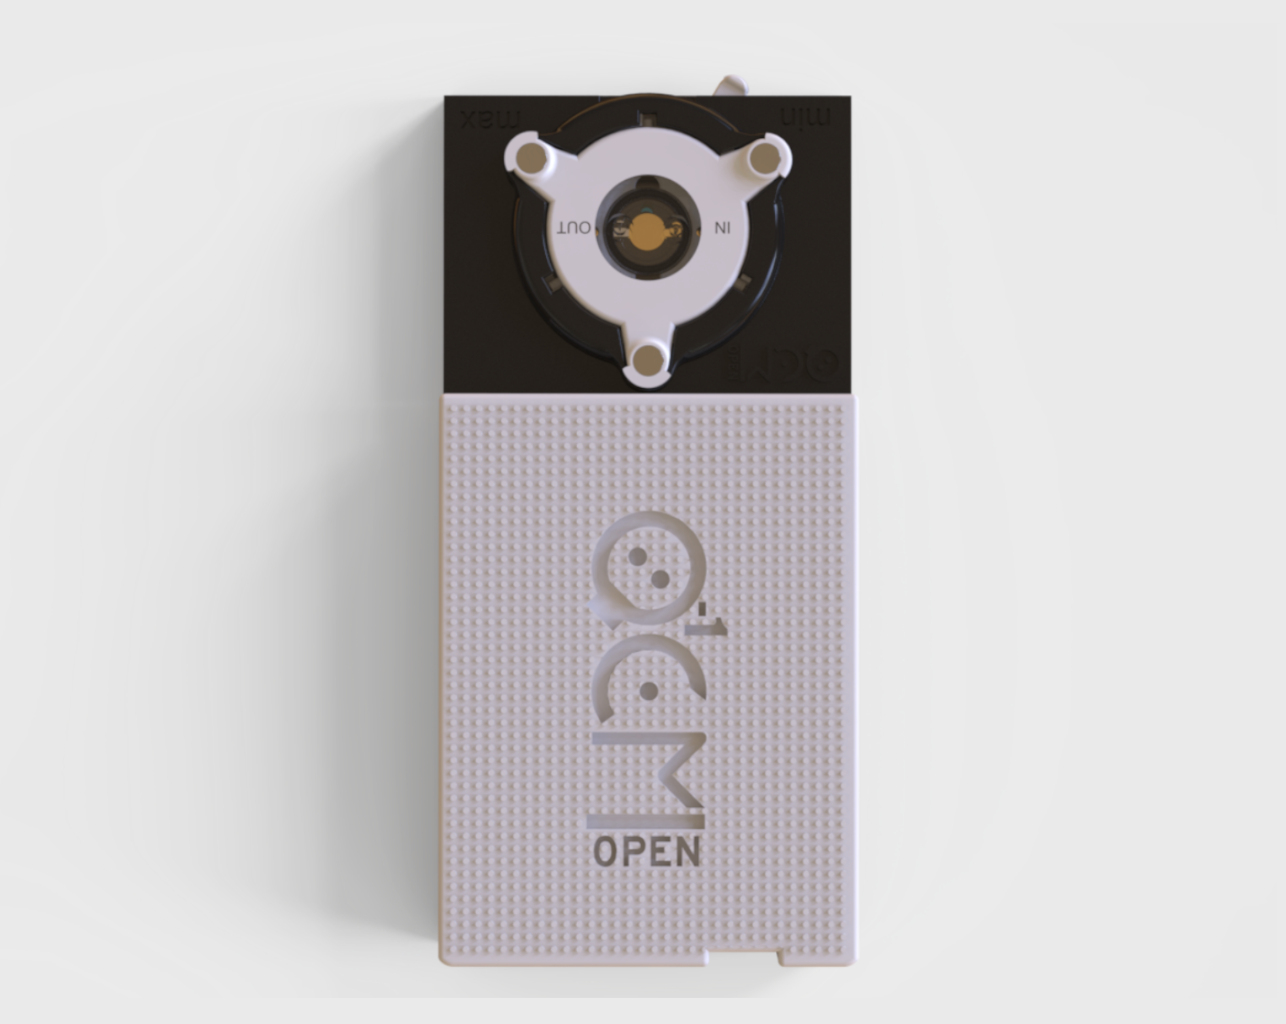
\includegraphics[width=\textwidth]{assets/figures/Quartz-Crystal-Microbalance-QCM-D-openQCM-Q-1.png}
    \caption{Capteur Q-1 de la société openQCM}
    \label{fig:Q-1}
\end{figure}

\section{Electroniques}
The electronics mainly consists of a scalar network analyser, the main block diagram is showed in
figure. The scheme of measurement follows the principle of passive interrogation of the quartz
sensor by sweeping around the resonance frequency.

\begin{figure}[H]
    \centering
    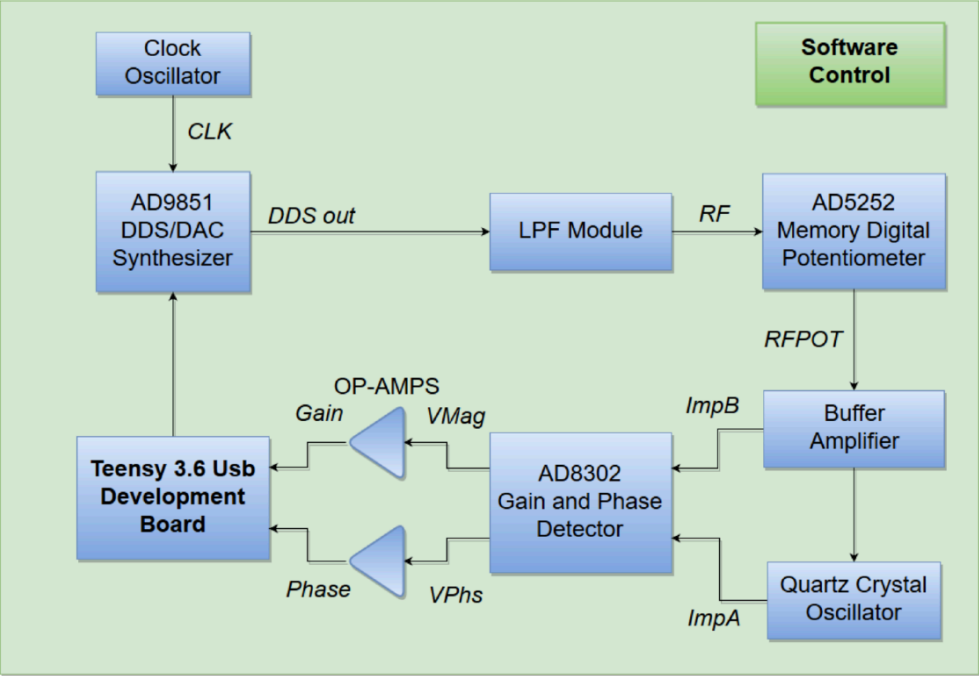
\includegraphics[width=\textwidth]{assets/figures/electronic block diagram QCM.png}
    \caption{diagramme bloc electronique du capteur Q-1}
    \label{fig:bloc diagram Q-1}
\end{figure}

\section{Carte mère}
\begin{figure}[H]
    \centering
    \begin{minipage}{0.48\textwidth}
        \small
        La carte mère est pilotée par une Teensy 3.6 (développée par Paul Stoffregen), 
        qui intègre un processeur ARM Cortex-M4. Cette carte se distingue par de nombreuses fonctionnalités, 
        dont la plus notable est l'entrée analogique (ADC) offrant une résolution réelle de 13 bits. 
        Cela signifie que, sur une plage pleine échelle de 3,3 volts, il est possible de mesurer des variations de tension d’entrée avec une résolution de 0,4 mV/bit \cite{manual-openqcmQ1}.
    \end{minipage}\hfill
    \begin{minipage}{0.48\textwidth}
        \centering
        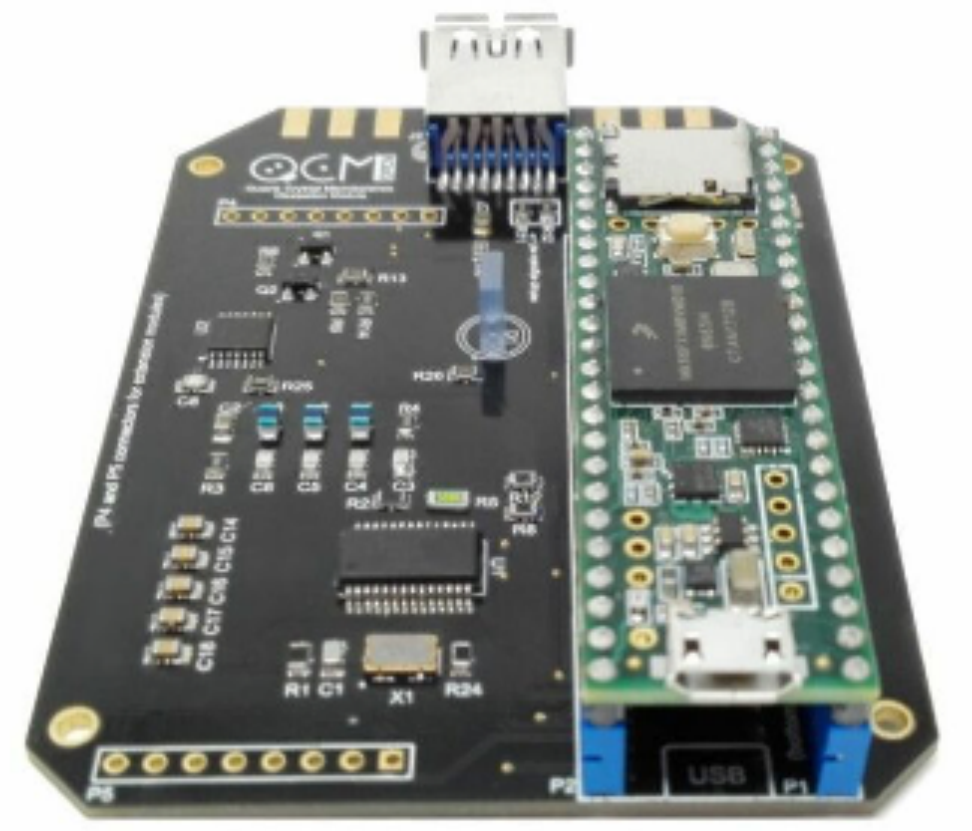
\includegraphics[width=\textwidth]{assets/figures/Quartz-Crystal-Microbalance-openQCM-Q-1-Shield-Photo.png}
        \caption{Diagramme bloc électronique du capteur Q-1}
        \label{fig:Main Board Q-1}
    \end{minipage}
\end{figure}

\section{cellules}
Les cellules de mesures ont pour but d'accueillir le cristal de quartz et le liquide à annalyser.
Elles possède un petit pcb qui fais le lien entre le cristal de quartz et la carte mère.
Ce PCB possède aussi un capteur de température pour mesurer la température de l'appareil de mesure.

\subsection{Cellule fluidique}
\begin{figure}[H]
    \centering
    \begin{minipage}{0.48\textwidth}
        \small
        La cellule de fluidique a comme spécificité d'avoir un petite chambre de mesures environ 50 µl.
        Le liquide traverse la chambre de mesure par deux orifices situé au dessus et en dessous du cristal. 
        si un pompe perisrataltique est utilisée,le liquide est asspier dans la chambre.
        Si un seringue est utilisée, le liquide est poussé dans la chambre.

        Un couvercle en plexiglas transparent permet de visualiser le cristal de quartz et le liquide à analyser,
        cepandant un autre couvercle en plastique est fourni pour des solvent qui peuvent endomager le plexiglas.
    \end{minipage}\hfill
    \begin{minipage}{0.48\textwidth}
        \centering
        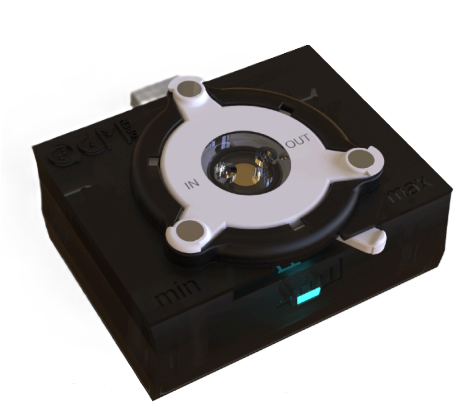
\includegraphics[width=\textwidth]{assets/figures/fluidic cell.png}
        \caption{Cellule de mesure du capteur Q-1}
        \label{fig:cellule de mesure Q-1}
    \end{minipage}
\end{figure}
\subsection{Cellule electrochimique}

\begin{figure}[H]
    \centering
    \begin{minipage}{0.48\textwidth}
        \small
        La cellule electrochimique est consure pour etre mesurer des reaction électrochimique.
        elle est composer d'un grand récippient de 10 ml, et un cristal de quartz au fond du récipient.
        La cellule n'est pas equipée des elecodes de la figure \ref{fig:cellule electrolitique Q-1}.
    \end{minipage}\hfill
    \begin{minipage}{0.48\textwidth}
        \centering
        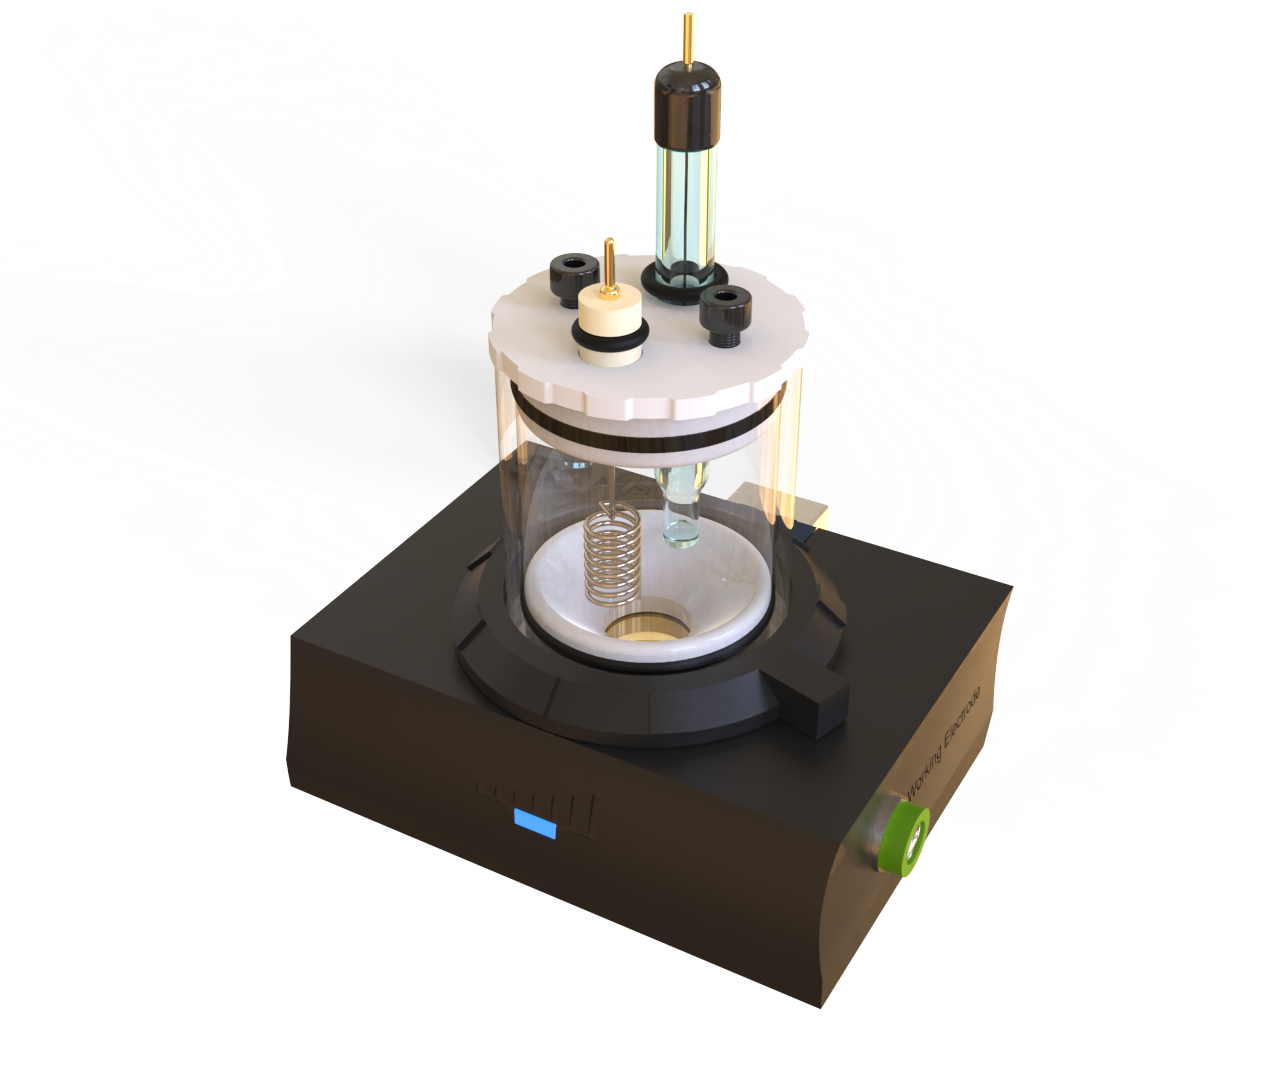
\includegraphics[width=\textwidth]{assets/figures/E-QCM_Module-openQCM-Q-1__71326.png}
        \caption{Cellule de mesure du capteur Q-1}
        \label{fig:cellule electrolitique Q-1}
    \end{minipage}
\end{figure}

\section{Software}
OpenQCM Q-1 GUI version 2.1 est une application open-source développée en Python par l'équipe openQCM et soutenue par Novaetech S.r.l. Ce logiciel est conçu pour afficher, traiter et stocker des données en temps réel provenant de l'appareil openQCM Q-1. Il est principalement destiné à un public scientifique, de recherche et d'ingénierie. L'installation nécessite le téléchargement de l'application depuis le site officiel, suivi de l'installation d'Anaconda3 pour Python 3.7. Des packages Python spécifiques comme pyqtgraph, pyserial, et h5py doivent être installés ou mis à jour via des commandes conda et pip. L'interface utilisateur principale se compose de trois fenêtres distinctes : "Setup/Control GUI", "Real-time Plot GUI" et "Info GUI", chacune offrant des fonctionnalités spécifiques pour le contrôle, la visualisation et l'information des données. Le logiciel permet également des procédures de calibration et de mesure, avec des options pour sauvegarder et exporter les données. Les graphiques en temps réel sont basés sur PyQtGraph, offrant des options interactives pour la visualisation et l'exportation des données.

\begin{figure}[H]
    \centering
    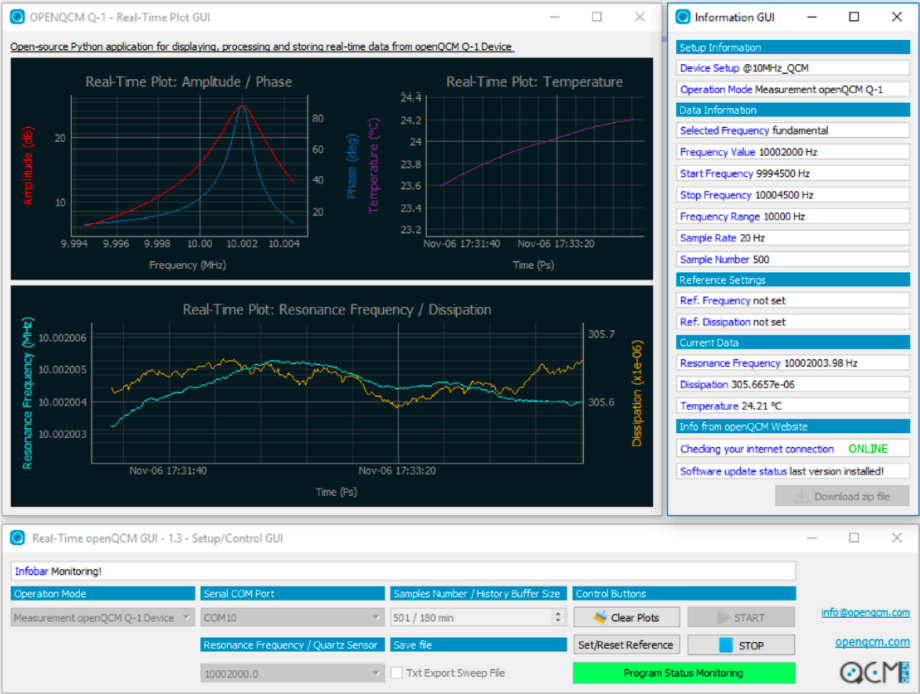
\includegraphics[width=\textwidth]{assets/figures/QCM-GUI.png}
    \caption{Application openQCM Q-1 GUI version 2.1}
    \label{fig:QCM-GUI}
\end{figure}